\documentclass[a4paper, openany, oneside, 11pt]{book} 
\usepackage[top=3cm, bottom=3cm, left=2.75cm, right=2.75cm]{geometry}

% structure packages
\usepackage{subfiles}
\usepackage[nottoc]{tocbibind}
\usepackage{makeidx} 
	\makeindex
\usepackage{enumitem}
\usepackage{fancyhdr} % fancy headder
	\setlength{\headheight}{15pt}
	\pagestyle{fancy}
	\renewcommand{\chaptermark}[1]{\markboth{#1}{}}
	\renewcommand{\sectionmark}[1]{\markright{#1}{}}
	\fancyhf{}
	\fancyhead[LE,RO]{\thepage}
	\fancyhead[LO]{{\nouppercase{\leftmark}}}
	\fancyhead[RE]{{\nouppercase{\leftmark}}} 
	\fancypagestyle{plain}{
	\fancyhf{} 
	\renewcommand{\headrulewidth}{0pt} 
	\renewcommand{\footrulewidth}{0pt}}

\usepackage{blindtext}
\usepackage{titlesec}
\usepackage{color}
    \definecolor{gray75}{gray}{0.75}
    \titleformat{\chapter}[hang]{\Huge\bfseries}{\thechapter\hspace{15pt}\textcolor{gray75}{$|$}\hspace{15pt}}{0pt}{\Huge\bfseries}

\setcounter{tocdepth}{4}
\setcounter{secnumdepth}{4}

% language settings
\usepackage[english,serbian]{babel}
\usepackage[utf8x]{inputenc} 
\usepackage[OT2,OT1]{fontenc} 
\usepackage[german=quotes]{csquotes}
\DeclareQuoteAlias{dutch}{serbian}

% character conversion settings
\renewcommand{\rmdefault}{wncyr} 
\renewcommand{\sfdefault}{wncyss}
\renewcommand{\encodingdefault}{OT2}

% figures, graphics \& plots
\usepackage[pdftex]{graphicx}
	\graphicspath{{res/}{../res/}}
\usepackage{wrapfig}
\usepackage{rotating}
\usepackage{caption}
\usepackage[list=true,listformat=simple]{subcaption} 
\usepackage{pgfplots}
\usepackage{pgfplotstable}

\usepackage{tikz}
\usetikzlibrary{calc,patterns,decorations.pathmorphing,decorations.markings}
\usetikzlibrary{arrows, shapes, calc, positioning, chains, backgrounds}
\usetikzlibrary{circuits.logic.US}
\tikzstyle{gnd}=[fill, pattern = north east lines, draw = none, minimum width = 1.00cm, minimum height = 0.05cm]
\usetikzlibrary{shadings, calc, decorations.markings}
\tikzset{->-/.style={decoration={markings,mark=at position #1 with {\arrow{>}}},postaction={decorate}},>-/.default=0.5,}

\usepackage{multirow}
\usepackage{pdflscape}
\usepackage{listings}
\usepackage{adjustbox}
\definecolor{codegreen}{rgb}{0,0.6,0}
\definecolor{codegray}{rgb}{0.5,0.5,0.5}
\definecolor{codepurple}{rgb}{0.58,0,0.82}
\definecolor{backcolour}{rgb}{0.95,0.95,0.92}
\lstdefinestyle{mystyle}{
    backgroundcolor=\color{backcolour},   
    commentstyle=\color{codegreen},
    keywordstyle=\color{purple},
    numberstyle=\tiny\color{codegray},
    stringstyle=\color{codepurple},
    basicstyle=\ttfamily\scriptsize,
    breakatwhitespace=false,         
    breaklines=true,                 
    captionpos=b,                    
    keepspaces=true,                 
    numbers=left,                    
    numbersep=5pt,                  
    showspaces=false,                
    showstringspaces=false,
    showtabs=false,                  
    tabsize=2
}
\lstset{style=mystyle}


\usepackage[title]{appendix}

% styles
\usepackage{tcolorbox}
\usepackage{color, colortbl}
\definecolor{Gray}{gray}{0.9}
\usepackage{lipsum}
\usepackage{hyperref} 
	\hypersetup{
	    colorlinks,
	    citecolor=black,
	    filecolor=black,
	    linkcolor=black,
	    urlcolor=blue
	}

% math packages
\usepackage{amsmath} 
\usepackage{amsfonts} 
\usepackage{amssymb} 
\usepackage{mathtools}
\usepackage{cancel}
\usepackage{tikz}
\usetikzlibrary{patterns}
\usepackage[siunitx]{circuitikz}
	\sisetup{output-decimal-marker = {,}}
\usepackage{mhchem}
\tikzset{
    partial ellipse/.style args={#1:#2:#3}{
        insert path={+ (#1:#3) arc (#1:#2:#3)}
    }
}
\def\centerarc[#1](#2)(#3:#4:#5)% Syntax: [draw options] (center) (initial angle:final angle:radius)
    { \draw[#1] ($(#2)+({#5*cos(#3)},{#5*sin(#3)})$) arc (#3:#4:#5); }
 \usepackage{soul}
 
% upright math operators
\DeclareMathOperator{\lin}{lin}
\DeclareMathOperator{\sgn}{sgn}

% chapter localization
\addto\captionsserbian{\renewcommand{\contentsname}{Sadrzhaj}} 
\addto\captionsserbian{\renewcommand{\bibname}{Literatura}}
\addto\captionsserbian{\renewcommand{\indexname}{Indeks pojmova}} 
\addto\captionsserbian{%
  \renewcommand\appendixname{Dodatak}
  \renewcommand\appendixpagename{Dodatak}
}
\setlength{\marginparwidth}{2cm}
\usepackage[]{todonotes}
\renewcommand{\chaptername}{}

\makeatletter
\providecommand*{\diff}%
{\@ifnextchar^{\DIfF}{\DIfF^{}}}
\def\DIfF^#1{%
\mathop{\mathrm{\mathstrut d}}%
\nolimits^{#1}\gobblespace}
\def\gobblespace{%
\futurelet\diffarg\opspace}
\def\opspace{%
\let\DiffSpace\!%
\ifx\diffarg(%
\let\DiffSpace\relax
\else
\ifx\diffarg[%
\let\DiffSpace\relax
\else
\ifx\diffarg\{%
\let\DiffSpace\relax
\fi\fi\fi\DiffSpace}

% Define block styles
\tikzstyle{decision} = [diamond, draw, fill=gray, 
    text width=4.5em, text badly centered, node distance=3cm, inner sep=0pt]
\tikzstyle{block} = [rectangle, draw, fill=gray, 
    text width=10em, text centered, rounded corners, minimum height=4em]
\tikzstyle{line} = [draw, -latex']
\tikzstyle{cloud} = [draw, ellipse,fill=red!20, node distance=3cm,
    minimum height=2em]

\bibliographystyle{ieeetr}

\begin{document}

\thispagestyle{empty}

\begin{center}
    \begin{Large}
        Univerzitet u Beogradu -- Elektrotehnichki fakultet \\ \vspace{5pt}
    \end{Large}
\end{center}

\vspace{100pt}
\begin{center}
	\begin{huge} \textbf{MASTER RAD} \end{huge} \\ 
        \vspace{10pt}
        na temu \\
        \vspace{10pt}
    \begin{huge} 
        \textbf{Sinteza video zapisa} \\ \vspace{-2pt}
        \textbf{na osnovu govornog signala upotrebom} \\ \vspace{-2pt}
        \textbf{rekurentnih neuralnih mrezha} \\
    \end{huge} 
\end{center}
\vspace{200pt}
\begin{center}
	\begin{large}
		kandidat: \hfill  mentor: \\ \vspace{5pt}
		Veljko Sheshelj, 3253/2018 \hfill doc. dr Predrag Tadic1
	\end{large}
\end{center}
\vfill
\begin{center}	
avgust, 2020.
\end{center}

\chapter*{Zahvalnica}
% \addcontentsline{toc}{chapter}{Zahvalnica}

\newpage
\tableofcontents

\newpage
\listoffigures
\chapter*{Uvod} 
\addcontentsline{toc}{chapter}{Uvod}
\markboth{Uvod}{Uvod}


\chapter{Obelezhja govora}
Prvi korak u sintezi lazhnog videa iz govora je odredjivanje karakteristichnih obelezhja govornog signala. Komponentne audio signala treba da su dovoljno dobre da nose lingvistichku komponentu, ali i da su otporne na pozadinski shum i na ostale smetnje.
Jedna od osnovnih pretpostavki vezanih za obradu govornog signala jeste da se govor mozhe prikazati kao izlaz linearnog, vremenski promenljivog sistema, chija se svojstva sporo menjaju sa vremenom. To vodi ka osnovnom principu analize govora koji kazhe da ako se posmatraju dovoljno kratki segmenti govornog signala, da se tada svaki segment mozhe modelirati kao izlaz linearnog, vremenski invarijantnog sistema \cite{OPGpredavanja}. Stoga se kratki segmenti govora mogu opisati konvolucionom jednachinom
\begin{equation}\label{eq:1.1}
s(t) = e(t)*\theta(t)
\end{equation}
pri chemu $s(t)$ predstavlja rezultatni govorni signal, $e(t)$ predstavlja pobudnu vazdushnu struju (eksitaciju) i $\Theta(t)$ impulsni odziv organa govornog trakta. U rachunarskoj obradi govora, signale je zgodnije posmatrati u diskretnom domenu
\begin{equation}
s[n] = e[n]*\theta[n]
\end{equation}
Zavisno od tipa eksitacije, govorni glasovi (fonemi) se mogu podeliti u tri distinktne kategorije:
\begin{itemize}[noitemsep]
\item zvuchni glasovi
\item frikativi (bezvuchni glasovi)
\item plozivi
\end{itemize}
Kod zvuchnih glasova, vazduh prelazi preko zategnutih glasnih zhica koje po\-chinju da vibriraju relaksiranim oscilacijama, proizvodec1i kvazi-periodichne chetvrtke koje c1e pobuditi vokalni trakt. Tipichni predstavnici zvuchnih glasova su samoglasnici. Pobuda koja proizvodi frikative je okarakterisana shirokim spektralnim sadrzhajem kao shto je sluchajni shum (glas \enquote{sh}). Plozivi nastaju pobudom koja je visokog inteziteta i kratkog trajanja (poput Dirakovog impulsa) (glasovi \enquote{b}, \enquote{p}, \enquote{t}...). Promenom oblika vokalnog trakta menja se frekvencijski sadrzhaj pobude i kao rezultat se dobijaju razlichiti fonemi. Engleski jezik razlikuje 42 fonema.\\
Problem govorne analize predstavlja odredjivanje parametara eksitacije i parametara implusnog odziva vokalnog trakta. Ovaj problem se mozhe nazvati i problemom razdvajanja konvolucionih komponenti, shto je poznato pod nazivom dekonvolucija.

\section{Kepstrum}
Kepstrum diskretnog signala $s[n]$ se mozhe izrachunati pomoc1u formule \cite{kepstrum}
\begin{equation}
c_s[n] = \boldsymbol{\mathcal{F}^{-1}}(\log(|\boldsymbol{\mathcal{F}}(s[n])|)
\end{equation}
gde su sa $\boldsymbol{\mathcal{F}}$ i $\boldsymbol{\mathcal{F}^{-1}}$ oznachene diskretna Furijeova transformacija (DFT) i inverzna DFT. Primenom DFT na jednachinu \ref{eq:1.1} dobija se
\begin{equation}
S(f) = E(f)\cdot\Theta(f)
\end{equation}
Izrachunavanje kepstruma mozhe se smatrati sistemom za dekonvoluciju zbog chinjenice da logaritam proizvoda dve komponetne predstavlja zbir logaritmovanih komponenti
\begin{align}
\log|S(f)| &= \log|E(f)\cdot\Theta(f)|\\
           &= \log|E(f)| + \log|\Theta(f)|\\
           &= C_E(f)+ C_{\Theta}(f)
\end{align}
Primenom inverzne Furijeove transformacije dobija se kepstrum govornog signala
\begin{align}
c_s[n] &= \boldsymbol{\mathcal{F}^{-1}}(C_E(f)+ C_{\Theta}(f))\\
       &= \boldsymbol{\mathcal{F}^{-1}}(C_E(f))+
       	  \boldsymbol{\mathcal{F}^{-1}}(C_{\Theta}(f))\\
       &= c_e[n]+ c_{\theta}[n]
\end{align}
U obliku signala $c_s[n]$ uochljive su oblasti u kojima dominiraju ekvivalenti vazdushne pobude  $c_e[n]$, odnosno impulsnog odziva govornih organa $c_{\theta}[n]$. Uticaj vazdushne pobude dominantniji je pri vec1im vrednostima argumenta, dok nizhe vrednosti argumenta nose informaciju o impulsnom odzivu vokalnog trakta. Zbog toga se najchesh\-c1e koristi prvih 12 kepstralnih koeficijenata, dok nulti koeficijent nosi informaciju o energiji signala.\\
Poshto je govor realan signal, amplituda spektra $|S(f)|$ je parna funkcija i kepstrum c1e imati realne vrednosti
\begin{align}
c_s[n] &= \boldsymbol{\mathcal{F}^{-1}}(\log(|\boldsymbol{\mathcal{F}}(s[n])|)\\
&=\frac{1}{N}\sum^{N-1}_{k=1}\log(|\boldsymbol{\mathcal{F}}(s[n])|)e^{\frac{j2kn\pi}{N}}\\
&=\frac{1}{N}\sum^{N-1}_{k=1}\log(|\boldsymbol{\mathcal{F}}(s[n])|)(\cos\left(\frac{2kn\pi}{N}\right)+j\sin\left(\frac{2kn\pi}{N}\right))\\
&=\frac{1}{N}\sum^{N-1}_{k=1}\log(|\boldsymbol{\mathcal{F}}(s[n])|)\cos\left(\frac{2kn\pi}{N}\right)
\end{align}
Zbog ovog svojstva, chesto se umesto inverzne diskretne Furijeove transoformacije koristi diskretna kosinusna transformacija radi smanjenja kompleksnosti izrachunavanja.

\section{Mel-frekvencijski kepstralni koeficijenti}
Prethodno opisani postupci se chesto koriste u primenama vezanim za automat\-sko prepoznavanje govora. U cilju oponashanja ljudskog nachina dozhivljavanja razlichitih uchestanosti u fonetima i primenjujuc1i kepstralnu analizu nastaju Mel-frekvencijski kepstralni koeficijnti (MFKK). 
\subsection{Melova frekvencijska skala}
Mel-skala je uskladjena sa ljudskim osec1ajem visine glasa odnosno njegove uchestanosti. Njeno dobijanje se vrshi eksperimentalno, slushaocu se reprodukuje ton uchestanosti $\SI{1000}{Hz}$ i kao njegovo zapazhanje o visini ovog tona se belezhi vrednost $\SI{1000}{mel}$, i ova vrednost se koristi kao mera uporedjivanja za dalje dobijanje mel skale. Zatim se uchestanost povec1ava sve dok slushalac ne primeti ton koji slusha ima duplo vec1u visinu od uporedne vrednosti i ta visina oznachava vrednosh\-c1u od $\SI{2000}{mel}$. Ovaj se princip dobija za dobijanje ostalih vrednosti skale. Eksperimenti su ipak pokazali da je medjusobna zavisnost mela i herca lienarna do $\SI{500}{Hz}$, dok iznad ove uchestanosti jednakim promenama mela odgovara sve vec1a promena u hercima. Za konvertovanje frekvencije u melovu skalu i nazad mogu se koristiti formule
\begin{equation}\label{freq2mel}
M(f) = 1125\log\left(1+\frac{f}{700}\right)
\end{equation}
\begin{equation}\label{mel2freq}
M^{-1}(m) = 700\left(\exp\left(\frac{m}{1125}\right)-1\right)
\end{equation}
\begin{figure}[h!]
\centering
  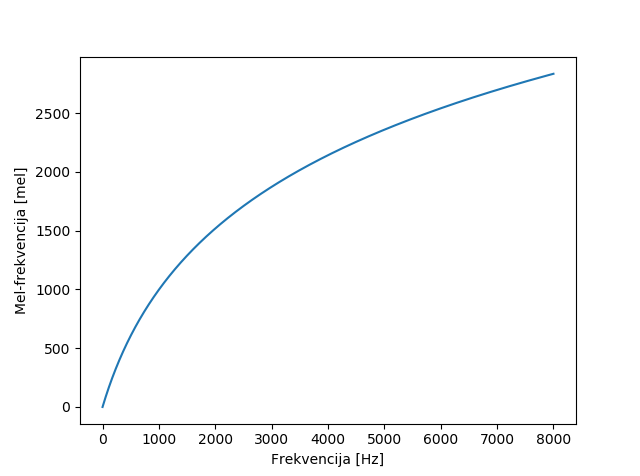
\includegraphics[scale=0.8]{res/freq2mel.png}
  \caption{Mel-frekvencijska skala}
  \label{fig:1}
  \vspace{0pt}
\end{figure}
\subsection{Melova banka filtara}
Postojanje auditornih kritichnih opsega je takodje osobina koja uslovljava ljudski dozhivljaj razlichitih uchestanosti. Ova pojava vezana je za chujni dozhivljaj slushaoca  prilikom slushanja dva razlichita tona na razlichitim uchestanostima. Dakle, ukoliko se slushocu pusti ton uchestanosti $f_1$ koja se nalazi u nekom chujnom opsegu, tada slushalac ima dozhivljaj tona u skladu sa mel sklaom. Ukoliko se pored tog tona pusti drugi ton uchestanosti $f_2$ tada zvuchni dozhivljaj slushaoca zavisi od medjusobne frekventne bliskosti ova dva tona. Naime, ukoliko je frekventni razmak dovoljno mali tako da se nalaze unutar istog kritichnog chujnog opsega dolazi do pojave maskiranja i slushalac chuje ton $f_1$, ali vec1e glasnosti. Ukoliko je frekventni razmak ovih tonova vec1i od shirine chujnog kritichnog opsega tada slushalac chuje dva tona na odgovarajuc1im prethodno pomenutim uchestanostima. Imajuc1i to u vidu frekvencijski opseg govornog signala potrebno je izdeliti na opsege. Ti opsezi formiraju melovu banku filtara. Postupak formitanja melove banke filtara se mozhe izdeliti na korake:
\begin{enumerate}
\item Koristec1i jendachinu \ref{freq2mel} konvertovati donju i gornju granicu govornog signala u melovu skalu. Za donju granicu se mozhe uzeti vrednost od $\SI{0}{Hz}$, dok je gornja frekvencija obichno uslovljena Nikvistovim kreiterijumom. U korish\-c1enom skupu podataka, govrni signal je odabiran sa $\SI{16}{kHz}$, pa je za gornju granicu korish\-c1ena vrednost od $\SI{8}{kHz}$.
\item Izdeliti opseg govornog signala na melovoj skali na ekvidistantne delove (opsege). Za broj delova se obichno uzima broj iz intervala $[26,\ 40]$. Za $n$ filtara dobijaju se $n+2$ frekvencije na melovoj skali.
\item Dobijene melove frekvencije, potrebno je vratiti u $\SI{}{Hz}$ frekvencije, formulom \ref{mel2freq}, koje se kasnije koriste za centralne uchestanosti trougaonih filtara
\end{enumerate}
\begin{figure}[h!]
\centering
  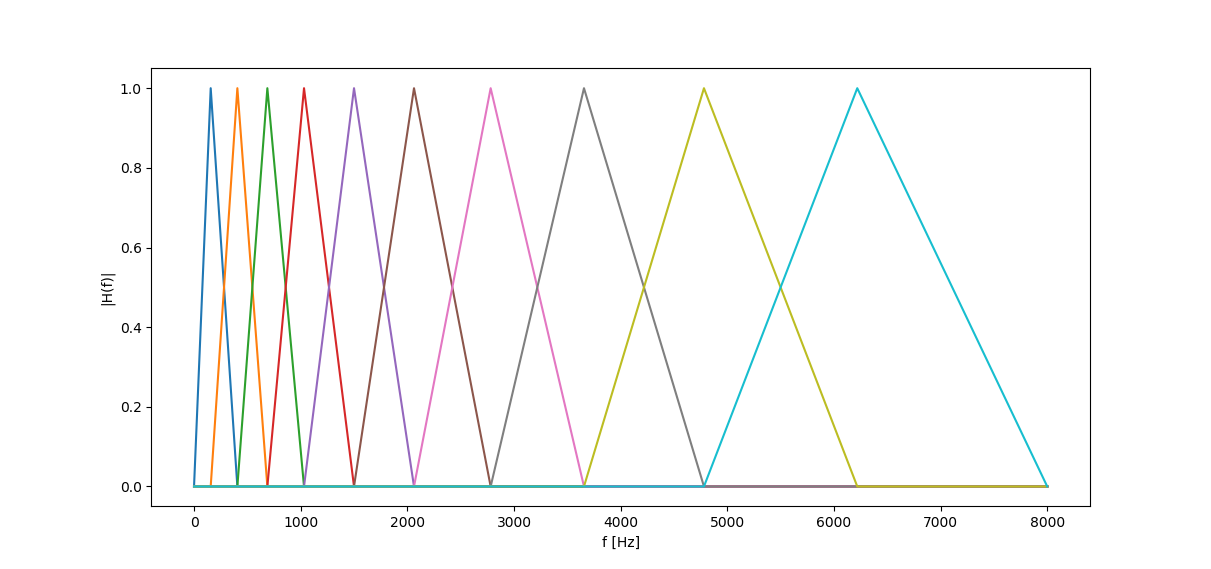
\includegraphics[scale=0.5]{res/10filterbank.png}
  \caption{Govorni frekvencijski opseg podeljen na 10 mel filtara}
  \label{fig:2}
  \vspace{0pt}
\end{figure}
\subsection{Algoritam izrachunavanja MFKK}
U ovom poglavlju c1e biti prikazan detaljan postupak dobijanja MFKK.
\begin{itemize}
\item \textbf{Visokofrekventno filtriranje}\\
Govorni signal je po prirodi analogni signal, koji je potrebno diskretizovati i digitalizovati da bi se izrachunala trazhena obelezhja. Pomenuti procesi su niskofrekventni i utichu na slabljenje vishih spektralnih komponenti u govornog signalu. Iz tog razloga nakon izvrshene digitalizacije, a pre samog izdvajanja obelezhja, potrebno je izvrshiti predobradu snimljenog govornog signala. To se postizhe primenom visokopropusnog filtra prvog reda
\begin{equation}
H(z) = 1-az^{-1}
\end{equation}
pri chemu se parametar $a$ bira iz intervala $[0.95,\ 0.98] $\cite{kepstrum}.
\item \textbf{Prozorovanje signala}\\
Na pochetku poglavlja je recheno da se samo kratki segmenti govora mogu smatrati kao izlaz linearnog, vremenski invarijantnog sistema. Sa tim u vezi signal je potrebno izdeliti na prozore duzhine $\SI{20}{ms}-\SI{40}{ms}$  \cite{OPGpredavanja}. U ovom radu izabrana je duzhina prozora od $\SI{25}{ms}$, sa preklapanjem izmedju susdenih prozora od $\SI{15}{ms}$. Naredni koraci se primenjuju za svaki prozor.
\item \textbf{Izrachunavanje spektra snage}\\
Za svaki prozor govornog signala je prvobitno potrebno odrediti DFT. Radi potiskivanja bochnih lobova, zgodno je primeniti Hamingov prozor pre izrachunavanja DFT. U ovom radu DFT se izrachunava u 512 tachaka. Spektar snage se mozhe estimirati periodogramom, koji za signal $s[n]$ se izrachunava po formuli
\begin{align}
S(f) &=\boldsymbol{\mathcal{F}}(s[n])\\
P(f) &=\frac{1}{N}|S(f)|^2
\end{align}
\item \textbf{Filtriranje spektra snage melovom bankom filtara}\\
Dobijeni periodogram je potrebno filtrirati kroz svaki filtar iz melove banke. Dobijeni koeficijenti za svaki filtar se sumiraju. Na kraju se dobijaju koeficijenti koji nam govore koliko je energije sadrzhano u svakom filtru filter banke.
\item \textbf{Logaritmovanje}\\
Logaritmovati svaki koeficijent dobijen propushtanjem periodograma kroz banku filtara.
\item \textbf{Diskretna kosinusna transformacija}\\
Diskretnom kosinusnom transformacijom nad logaritmovanim energijama dobijaju se kepstralni koeficijenti.
\end{itemize}
\subsection{Dinamichka obelezhja}
Chesto je od interesa posmatrati i promenu MFKK u vremenu \cite{kepstrum}. Na ovaj nachin, korish\-c1ena obelezhja direktno nose informaciju o promenama izmedju susednih prozora govornog signala. Radi izrachunavanja ovih obelezhja koriste se polinomijalne aproksimacije prvog i drugog izvoda kepstralnih koeficijenata \cite{MFKKlink}
\begin{align}
\Delta c_t &= \frac{\sum^{N}_{n=1}n(c_{t+n}-c_{t-n})}{2\sum^{N}_{n=1}n^2}\\
\Delta^2 c_t &= \frac{\sum^{N}_{n=1}n(\Delta_{t+n}-\Delta_{t-n})}{2\sum^{N}_{n=1}n^2}
\end{align}
gde su $\Delta c_t$ i $\Delta^2 c_t $ delta i delta-delta kepstralni koeficijenti za prozor $t$, izrachunati iz statichkih kepstralnih koeficijenata iz okolnih prozora. Tipichna vrednost koja se uzima je $N=2$.
\section{Prikaz obelezhja govora}
U ovom radu, kao vektor ulaznih parametara, korish\-c1eno je 13 kepstralnih koeficijenata, sa njihom deltama, shto daje ulazni vektor dimenzije 26. Umesto prvog kepstra, korish\-c1ena je energija signala. Iz baze video fajlova, samo audio snimci su izvucheni uz pomoc1 alata $FFmpeg$ \cite{FFmpeg}, chime se dobija baza audio snimaka govora predsednika Obame. Nakon toga, svaki video je normalizovan uz pomoc1 $FFmpeg-normalize$ dodatka \cite{FFmpegN}. Prikaz nekih kepstralnih koeficijenata, za nasumichno odabran audio snimak iz baze, se mozhe pogledati u nastavku.
\begin{figure}[h!]
\centering
  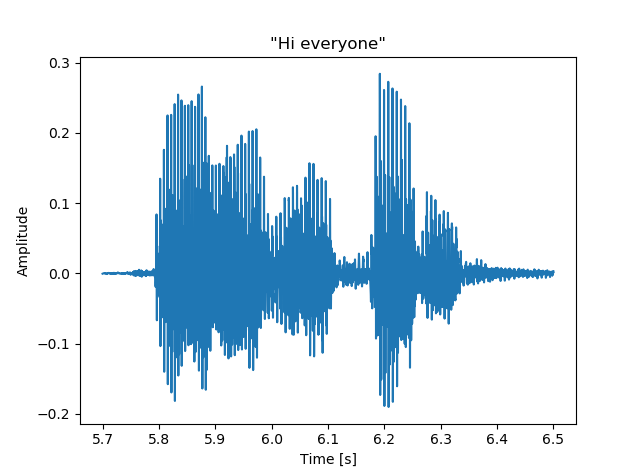
\includegraphics[scale=0.5]{res/audio_sig.png}
  \caption{Nasumichni noramlizovani audio signal iz baze}
  \label{fig:3}
  \vspace{0pt}
\end{figure}
\begin{figure}[!h]
        \centering
        \begin{subfigure}{0.475\textwidth}
            \centering
            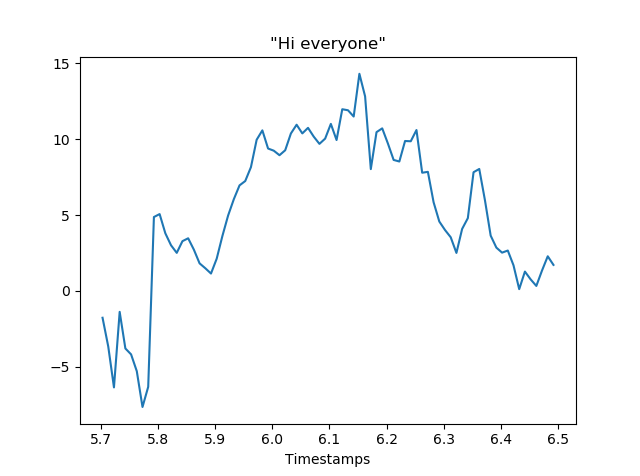
\includegraphics[scale=0.5]{res/cep1.png}
            \caption{Prvi MFKK}
            \label{fig:4a}
            \vspace{0pt}
        \end{subfigure}%
        \begin{subfigure}{0.475\textwidth}
            \centering
            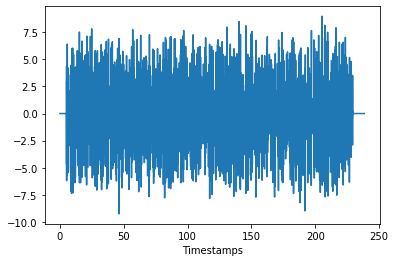
\includegraphics[scale=0.5]{res/Dcep1.png}
            \caption{Delta prvog MFKK}
            \label{fig:4b}
            \vspace{0pt}
        \end{subfigure}
        \caption{Prikaz glasovnih obelezhja}
        \label{fig:4}
\end{figure}
\newpage
\begin{figure}[!h]
        \centering
        \begin{subfigure}{0.475\textwidth}
            \centering
            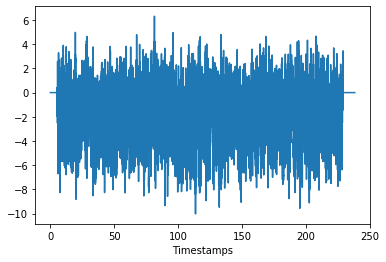
\includegraphics[scale=0.5]{res/cep6.png}
            \caption{Shesti MFKK}
            \label{fig:5a}
            \vspace{0pt}
        \end{subfigure}%
        \begin{subfigure}{0.475\textwidth}
            \centering
            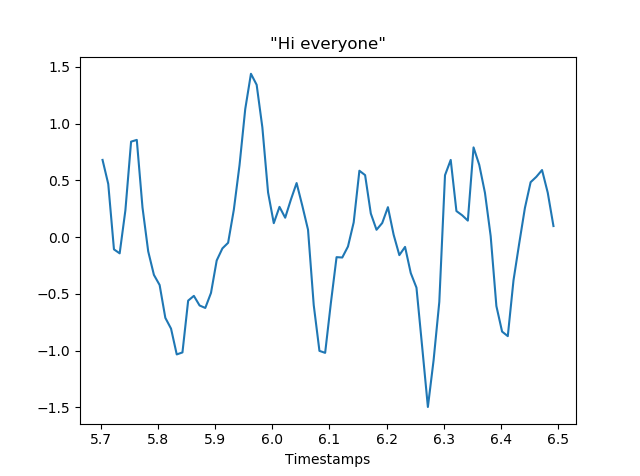
\includegraphics[scale=0.5]{res/Dcep6.png}
            \caption{Delta shestog MFKK}
            \label{fig:5b}
            \vspace{0pt}
        \end{subfigure}
        \caption{Prikaz glasovnih obelezhja}
        \label{fig:5}
\end{figure}
\begin{figure}[!h]
        \centering
        \begin{subfigure}{0.475\textwidth}
            \centering
            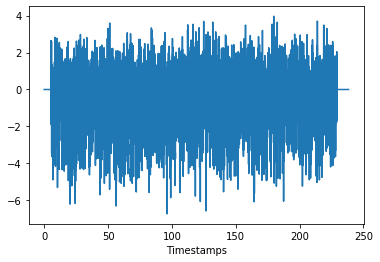
\includegraphics[scale=0.5]{res/cep12.png}
            \caption{Dvanaesti MFKK}
            \label{fig:6a}
            \vspace{0pt}
        \end{subfigure}%
        \begin{subfigure}{0.475\textwidth}
            \centering
            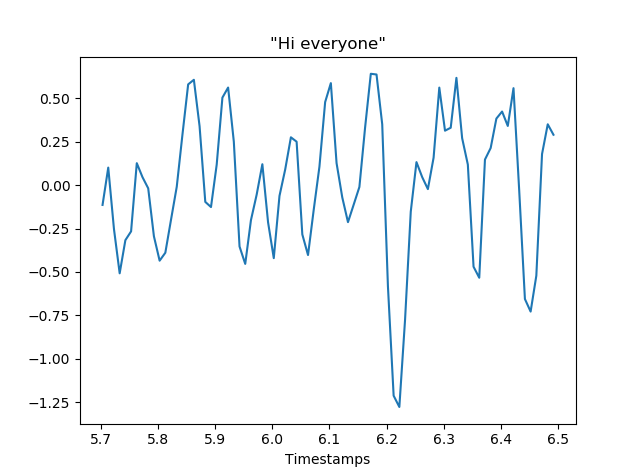
\includegraphics[scale=0.5]{res/Dcep12.png}
            \caption{Delta dvanaestog MFKK}
            \label{fig:6b}
            \vspace{0pt}
        \end{subfigure}
        \caption{Prikaz glasovnih obelezhja}
        \label{fig:6}
\end{figure}

\chapter{Obelezhja videa}

\chapter{Rekurentne neuralne mrezhe}
Neuralne mrezhe su modeli uchenja koji ostvaraju ogroman uspeh u shirokom spektru zadataka superviziranog i nesuperviziranog mashinskog uchenja. Klasichne ($feedforward$) neuralne mrezhe se posebno izdvajaju u problemima klasifikacije. Uprkos njihovoj moc1i, standardne neuralne mrezhe imaju ogranichenja, od kojih je naznachajnije da primeri iz baze podataka moraju biti medjusobno nezavisni. U sluchaju kada su podaci zavisni u vremenu i prostoru ovo nije prihvatljivo. Frejmovi videa, delovi audio signala, rechi iz rechenice predstavljaju primere podataka gde zahtev o medjusobnoj nezavisnosti nije zadovoljen. Rekurentne neuralne mrezhe prevazilaze taj nedostatak i koriste se u sluchahevima kada se podaci mogu prikazati u formi sekvence. One imaju osobinu da selektivno prosledjuju informaciju izmedju koraka sekvence, dok i dalje procesuju jedan po jedan korak.\\
U ovom poglavlju c1e se prvo baciti kratak osvrt na klasichne ($feedforward$) neuralne mrezhe, a zatim c1e biti detaljnije obradjen pojam razlichitih vrsta rekurentnih neuralnih mrezha.

\section{Pregled veshtachkih neuralnih mrezha}
Neuralne mrezhe su modeli izrachunavanja inspirasni bioloshkim neuralnim sistemom. Neuralna mrezha se sastoji od skupa veshtachkih neurona, koji se josh i nazivaju chvorovima, koji su medjusobno povezani sinapsama (vezama). Za svaki neuron $j$ se definishe funkcija aktivacije $l_j(*)$ i integraciona funkcija $f_j(*)$. Veza od chvora $j'$ ka chvoru $j$ je opisana tezhinskim koeficijentom $w_{jj'}$.
\begin{figure}[!h]
\hspace*{0.1\linewidth}
\begin{tikzpicture}
	\tikzstyle{rectangle_style}=[rectangle, draw]
	\tikzstyle{dividedrectangle_style}=[draw, rectangle split, rectangle split parts=2, rotate = 90, minimum height = 15mm, minimum width = 10mm]
	% neuron i
	\foreach \x in {0,...,2}
		\draw node at (0, -\x) [rectangle_style] (neuron_i_\x) {$v_\x$};
	\foreach \x in {1,...,3}
		\fill (0, -2.5 - \x*0.15) circle (1pt);
	\draw node at (0, -3.5) [rectangle_style] (neuron_i_3) {$v_i$};
	% w_ji
	\foreach \x in {0,...,2}
		\draw node at (1.5, -\x) [] (w_ji_\x) {$w_{j\x}$};
	\draw node at (1.5, -3.5) [] (w_ji_i) {$w_{ji}$};
	\foreach \x in {1,...,3}
		\fill (1.5, -2.5 - \x*0.15) circle (1pt);
	% neuron j
	\node at (6.5, -1.5) [dividedrectangle_style] (neuron_j){\rotatebox{-90}{$s_j = f_j (w_{ji}v_i)$} \nodepart{second} \rotatebox{-90}{$v_j = l_j (s_j)$}};
	% error
	\node at (10, -1.5) [] (error) {$v_j$};
	% connect: y_i -> w_ji
	\foreach \i in {0,...,2}
		\path[-] (neuron_i_\i) edge node[] {} (w_ji_\i);
	\path[-] (neuron_i_3) edge node[] {} (w_ji_i);
	\begin{scope}[decoration={
    markings,
    mark=at position 0.5 with {\arrow{>}}}
    ] 
	% connect: w_ji -> neuron j
	\foreach \i in {0,...,2}
		\draw[postaction={decorate}] (w_ji_\i) -- (neuron_j.north);
	\draw[postaction={decorate}] (w_ji_i)--(neuron_j.north);
	\end{scope}
	% connect: neuron j -> output
	\path[->] (neuron_j) edge node[above, midway] {$ $} (error);
\end{tikzpicture}
\caption{Shemat\-ski prikaz veshtachkog neurona}
\label{fig:7}
\end{figure}\\
Za integracionu funkciju se najchesh\-c1e uzima linearna suma, te se vrednost na izlazu jednog chvora mozhe izrachunati kao
\begin{equation}\label{node}
v_j = l_j\left(\sum^{i}_{k=0}w_{ji}v_i\right)
\end{equation}
Chesti izbori aktivacione funckije su sigmoid $\sigma(z)=1/(1+e^{-z})$ i hiperbolichki tangens $\tanh(z) = (e^z-e^{-z})/(e^z-e^{-z})$. Od skora, u modelima dubokih neuralnih mrezha koristi se aktivaciona funkcija $ReLU(z)=max(0,z)$ koja je pokazala zna\-chajno poboljshanje performansi.\\
$Feedforward$ neurlne mrezhe su vrsta veshtachkih neuralnih mrezha chiji usmereni grafovi ne smeju da sadrzhe petlje. Zbog odsustva petlji, chvorove  mrezhe je moguc1e organizovati u slojeve. Izlaz jednog sloja se dobija na osnovu izlaza nizhih slojeva.
\begin{figure}[h]
\begin{center}
    \begin{tikzpicture}
    	\tikzstyle{place}=[circle, draw=black, minimum size = 8mm]
    	
    	% Input
    	\foreach \x in {1,...,3}
    		\draw node at (0, -\x*1.25) [place] (first_\x) {$x_\x$};
    	\foreach \x in {1,...,3}
    		\fill (0, -4.5 -\x*0.3) circle (2pt);
    	\draw node at (0, -5*1.25) [place] (first_n) {$x_n$};
    	
    	% Hidden 1
    	\foreach \x in {1,...,3}
    		\node at (4, -\x*1.25) [place] (second_\x){$a_\x$};
    	\foreach \x in {1,...,3}
    		\fill (4, -4.5 -\x*0.3) circle (2pt);
    	\draw node at (4, -5*1.25) [place] (second_m) {$a_m$};
    	
    	% Output
	\foreach \x in {1,...,3}
    		\node at (8, -\x*1.25) [place] (fourth_\x){$y_\x$};
	\foreach \x in {1,...,3}
    		\fill (8, -4.5 -\x*0.3) circle (2pt);
    	\node at (8, -5*1.25) [place] (fourth_m) {$y_k$};
    		
    	% Input -> Hidden
    	\foreach \i in {1,...,3}
    		\foreach \j in {1,...,3}
    			\draw [->] (first_\i) to (second_\j);
    	\foreach \i in {1,...,3}
    		\draw [->] (first_\i) to (second_m);
    	\foreach \i in {1,...,3}
    		\draw [->] (first_n) to (second_\i);
	\draw [->] (first_n) to (second_m);
    	
    	% Hidden -> Output
    	\foreach \i in {1,...,3}
		\foreach \j in {1,...,3}
    			\draw [->] (second_\i) to (fourth_\j);
	\foreach \i in {1,...,3}
    		\draw [->] (second_\i) to (fourth_m);
    	\draw [->] (second_m) to (fourth_m);
    	
    	% Text
    	\node at (0, -8) [black, ] {Ulazni sloj};
    	\node at (4, -8) [black, ] {Skriveni sloj};
    	\node at (8, -8) [black, ] {Izlazni sloj};
    \end{tikzpicture}
    \caption{Shemtaski prikaz visheslojne $feedforward$ neuralne mrezhe}
    \label{fig:8}
\end{center}
\end{figure}\\
Vektor obelezhja $\mathbf{x}$ se dovodi na najnizhi (ulazni) sloj. Izlazi chvorova u narednim slojevima se sukcesivno izrachunavaju, dok se ne dobije izlaz najvisheg (izlaznog) sloja mrezhe $\mathbf{\hat{y}}$. $Feedforward$ mrezhe se koriste u supervizovanom uchenju na zadacima klasifikacije i regresije. Uchenje se ostvaruje azhuriranjem tezhinskih koeficijenata $w_{jj'}$ sa ciljem da se optimizuje kriterijumska funkcija $\mathfrak{L}(\mathbf{\hat{y}}, \mathbf{y})$, koja penalizuje distancu izmedju izlaznog vektora $\mathbf{\hat{y}}$ i vektora cilja $\mathbf{y}$.\\
Najuspeshniji algoritam za traniranje neuralnih mrezha je algoritam propagacije u nazad (eng. $backpropagation$)\cite{Backprog}. Algoritam propagacije u nazad koristi lanchano pravilo za rachunanje izvoda kriterijumske funkcije $\mathfrak{L}$. Tezhinski koeficijenti se popravljaju koristec1i algoritam gradijentnog spusta. Najchesh\-c1e korish\-c1en algoritam gradijentnog spusta je gradijentni spust koji koristi mini šarže (eng. $batch$) obuchavajuc1eg skupa. Taj algoritam kombinuje prednosti sharzhnog i stohastichkog gradijentnog spusta. Primenom tog algoritma koeficijenti se azhuriraju na osnovu akumulirane greshke svih primeraka iz mini sharzhe. Za sharzhu duzhine $n$ pravilo azhuriranja tezhinskih koeficijenata se mozhe zapisati ovako
\begin{equation}\label{SGD}
w := w- \eta\nabla_w\mathfrak{L}\left(\mathbf{\hat{y}^{i:i+n}}, \mathbf{y^{i:i+n}}\right)
\end{equation}
gde je sa $\eta$ oznachena brzina obuchavanja (eng. $learning\ rate$).
U opstem sluchaju, kriterijumska funkcija nije konveksna, i ne postoji garant da c1e gradijentni spust dovesti do globalnog minimuma. Mnoge varijante gradijentnog spusta se uvode kako bi se ubrzalo obuchavanje. Neke od najpopularnijih su: $AdaDelta$ \cite{AdaDelta}, $AdaGrad$ \cite{AdaGrad}, $RMSprop$ \cite{RMSprop} i $Adam$ \cite{Adam}. Uglavnom se zasnivaju na menjanju brzine obuchavanja kao i na momentumu koji predstavlja promenu tezhinskog koeficijenta u prethodnoj iteraciji algoritma.\\
Da bi se izrachunao gradijent u jednachini \ref{SGD} koristi se, vec1 pomenut, algoritam propagacije u nazad. Kao shto joj samo ime kazhe, algoritam zapochinje od izlaznog sloja i krec1e unazad ka nizhim slojevima. 
Za chvor $j$, koji se nalazi u izlaznom sloju, aktivacione funkcije $l_j(*)$ i linearnom integracionom funcijom $s_j(*)$, vazhi jednachina \ref{node}
\begin{align}
y_j=v_j &= l_j\left(s(w_{ji},v_i)\right)\\
&=l_j\left(\sum^{i}_{k=0}w_{ji}v_i\right)
\end{align}
Za tezhinski koeficijent veze izmedju chvora $j$ iz izlaznog sloja i cvora $i$ iz skrivenog sloja, promena se mozhe dobiti na sledec1i nachin
\begin{align}
\Delta w_{ji} &= -\eta\frac{\partial \mathfrak{L}\left(\mathbf{\hat{y}}, \mathbf{y}\right)}{\partial w_{ji}}\\
&=-\eta\left[\frac{\partial \mathfrak{L}\left(\mathbf{\hat{y}}, \mathbf{y}\right)}{\partial y_j}\right]\left[\frac{\partial y_j}{\partial s(w_{ji},v_i)}\right]\left[\frac{\partial s(w_{ji},v_i)}{\partial w_{ji}}\right]\\
&=\eta \delta_{ji}v_h\\
\delta_{ji} &=-\left[\frac{\partial \mathfrak{L}\left(\mathbf{\hat{y}}, \mathbf{y}\right)}{\partial y_j}\right]\left[\frac{\partial y_j}{\partial s(w_{ji},v_i)}\right] \label{delta}\\
&= -\left[\frac{\partial \mathfrak{L}\left(\mathbf{\hat{y}}, \mathbf{y}\right)}{\partial y_j}\right]l'_j(s_j)
\end{align}
Velichina $\delta_{ji}$ se naziva i signalom greshke. Prvi chinilac u izrazu \ref{delta} zavisi od izbora kriterijumske funkcije, a drugi predstavlja izvod aktivacione funkcije $l'_j(*)$. Za tezhinski koeficijent veze izmedju chvora koji pripada skrivenom sloju $i$ i chvora koji se nalazi u sloju iza $l$ vazhi
\begin{align}
\Delta w_{il} &= -\eta\frac{\partial \mathfrak{L}\left(\mathbf{\hat{y}}, \mathbf{y}\right)}{\partial w_{il}}\\
&=-\eta\left[\frac{\partial \mathfrak{L}\left(\mathbf{\hat{y}}, \mathbf{y}\right)}{\partial v_i}\right]\left[\frac{\partial v_i}{\partial s_l}\right]\left[\frac{\partial s_l}{\partial w_{il}}\right]\\
&=\eta \delta_{il}v_l\\
\delta_{il} &= l'_l(s_l)\sum_{k}\delta_{kl}w_{kl}\label{delta1}
\end{align}
Jednachina \ref{delta1} se sukcesivno primenjuje za sve nizhe slojeve, chime se uz sachuvane vrednosti izlaza chvorova dobijaju gradijenti pojedinachnih tezhinskih koeficijenata.

\section{Rani modeli rekurentnih neuralnih mrezha}
Rekurentne neuralne mrezhe su mrezhe chiji usmereni grafovi dozovljavaju petlje, chime se uvodi pojam vremena u model. U trenutku $t$, chvorovi sa rekurentnim vezama zavise od trenutnog ulaznog vektora $\mathbf{x}^{(t)}$ i vrednosti stanja chvora u prethodnom trenutku $\mathbf{h}^{(t-1)}$. Izlaz chvora $\mathbf{\hat{y}^{(t)}}$, zavisi od vrednosti stanja chvora $\mathbf{h}^{(t)}$ i posredstvom rekurentnih veza ulaz ulaz u trenutku $t-1$ 
$\mathbf{x}^{(t-1)}$ mozhe uticati na izlaz u trenutku $t$.
\newpage
\begin{figure}[!h]
\hspace*{0.1\linewidth}
\begin{tikzpicture}[item/.style={circle,draw,thick,align=center},
itemc/.style={item,on chain,join}]
 \begin{scope}[start chain=going right,nodes=itemc,every join/.style={-latex,very thick},local bounding box=chain]
 \path node (A0) {$\mathbf{h}^0$} node (A1) {$\mathbf{h}^{1}$} node (A2) {$\mathbf{h}^{2}$} node[xshift=2em] (At){$\mathbf{h}^{t}$};
 \end{scope}
 \node[left=1em of chain,scale=2] (eq) {$=$};
 \node[left=2em of eq,item] (AL) {$\mathbf{h}$};
 \path (AL.west) ++ (-1em,2em) coordinate (aux);
 \draw[very thick,-latex,rounded corners] (AL.east) -| ++ (1em,2em) -- (aux) 
 |- (AL.west);
 \foreach \X in {0,1,2,t} 
 {\draw[very thick,-latex] (A\X.north) -- ++ (0,2em)
 node[above,item,fill=gray!10] (h\X) {$\mathbf{y}^\X$};
 \draw[very thick,latex-] (A\X.south) -- ++ (0,-2em)
 node[below,item,fill=gray!10] (x\X) {$\mathbf{x}^\X$};}
 \draw[white,line width=0.8ex] (AL.north) -- ++ (0,1.9em);
 \draw[very thick,-latex] (AL.north) -- ++ (0,2em)
 node[above,item,fill=gray!10] {$\mathbf{y}^t$};
 \draw[very thick,latex-] (AL.south) -- ++ (0,-2em)
 node[below,item,fill=gray!10] {$\mathbf{x}^t$};
 \path (x2) -- (xt) node[midway,scale=2,font=\bfseries] {\dots};
\end{tikzpicture}
\caption{Shemat\-ski prikaz odmotane rekurentne neuralne mrezhe u vremenu}
\label{fig:9}
\end{figure}
Mrezha sa slike \ref{fig:9} se mozhe opisati jednachinama
\begin{align}
\mathbf{h}^t &= l_h(\mathbf{W_{hx}}\mathbf{x}^t+\mathbf{W_{hh}}\mathbf{h}^{t-1}+\mathbf{b_h})\label{RNN1}\\ 
\mathbf{y}^t &= l_y(\mathbf{W_{yh}}\mathbf{h}^t+\mathbf{b_y})\label{RNN2}
\end{align}
gde su sa $\mathbf{W_{hx}}$, $\mathbf{W_{yh}}$ i $\mathbf{W_{hh}}$ matrice koje sadrzhe tezhinske koeficijente, a $l_h$ i $l_y$ neke aktivacione funkcije. Vektori $b_h$ i $b_y$ omoguc1avaju uchenje ofseta.\\
Istrazhivanja na temu rekurentnih neuralnih mrezha su zapochela osadesetih godina prošloga veka. Prvo je Hopfild predstavio familiju rekurentnih neuralnih mrezha koja je imala moguc1nosti prepoznavanja shablona \cite{Hopfild}. Struktura mrezhe je ista kao na slici \ref{fig:9}, s tim da se ulazni shablon $\mathbf{x}$ primeni samo u pochetnom trenutku, nakon koga se mrezha prepusti izrachunavanjima  sve dok se na izlazu ne dobije stacionarna vrednost. Hopfildove mrezhe imaju moguc1nost da reprodukuje memorisane shablone iz zashumljenih shablona koje dobiju na ulazi i predstavljaju pretechu Bolcmanovih mashina i auto-enkodera.\\
Rani model za supervizovano uchenje sekvenci je predstavio D2ordan u \cite{jordan}. Model je $feedforward$ mrezha koja se sastoji od jednog skrivenog sloja koji sadrzhi specijalne chvorove. Izlaz mrezhe je vezama spojen sa specijalnim chvorovima, koji rekurentnim vezama, u narednom vremenskom trenutku, dostavljaju vrednosti ostalim chvorovima skrivenog sloja. U sluchaju da izlaz mrezhe predstavlja neke akcije, ovakav model omoguc1ava pamec1enje akcije iz prethodnog vremensog trenutka. Nekoliko modernih modela koristi ovu ideju. Jedan takav primerak je rad \cite{Sutskever} gde se na primeru prevodioca jezika, pri generisanju teksta prevedenih rechenica, rechi sa kraja se vrac1aju i koriste kao ulaz za naredni korak. Specijalni chvorovi mogu da sadrzhe i dodatnu rekurentnu vezu tako da za ulaz imaju i svoje prethodno stanje (slika \ref{fig:10}).\\
Elmanov model iz \cite{Elman} predstavlja arhitekturu koja lichi na mrezhu sa slike \ref{fig:9}. Za razliku od D2ordanovog modela, koji chuva trenutnu vrednost izlaza u specijalnim chvorovima, Elmanov model chuva trenutnu vrednost chvorova skrivenog sloja, koju u narednom vremenskom trenutku vrac1a tim skrivenim chvorovima (slika \ref{fig:11}). Elman je u svom radu trenirao mrezhu algoritmom propagacije u nazad i dokazao da mrezha mozhhe nauchiti zavisnosti od vremena.
\newpage
\begin{figure}[!h]
\hspace*{0.4\linewidth}
\begin{tikzpicture}[item/.style={circle,draw,thick,align=center}]
 \node[left=0,item, inner sep=2pt, minimum size=1cm] (AL) {$\mathbf{h}$};
 
 \draw[white,line width=0.8ex] (AL.north) -- ++ (0,1.9em);
 \draw[very thick,-latex] (AL.north) -- ++ (0,2em)
 node[above,item,fill=gray!10,inner sep=2pt, minimum size=1cm](y) {$\mathbf{y}^t$};
 \draw[very thick,latex-] (AL.south) -- ++ (0,-2em)
 node[below,item,fill=gray!10,inner sep=2pt, minimum size=1cm] {$\mathbf{x}^t$};
 
 \node[right=1cm, item,inner sep=2pt, minimum size=1cm](s) {$\mathbf{s}$};
 \draw[very thick,-latex, dotted] (s.west) to [out=-150,in=-30] (AL.east);
 \draw[very thick,-latex, red](y.east) to (s.north);
 \draw[very thick,-latex,dotted](s.east) to [out=0,in=-90,distance=2cm](s.south);
 \node[text width=4cm] at (5,2)(t1) {rekurentna veza};
 \draw [very thick,-latex,dotted] (2,2.05) to (3,2.05);
 \node[text width=4cm] at (5,1.5)(t2) {$\mathbf{W}=1$};
 \draw [very thick,-latex, red] (2,1.54) to (3,1.54);
\end{tikzpicture}
\vspace{0pt}
\caption{Shemat\-ski prikaz D2ordanovog modela}
\label{fig:10}
\end{figure}
\begin{figure}[!h]
\hspace*{0.4\linewidth}
\begin{tikzpicture}[item/.style={circle,draw,thick,align=center}]
 \node[left=0,item, inner sep=2pt, minimum size=1cm] (AL) {$\mathbf{h}$};
 
 \draw[white,line width=0.8ex] (AL.north) -- ++ (0,1.9em);
 \draw[very thick,-latex] (AL.north) -- ++ (0,2em)
 node[above,item,fill=gray!10,inner sep=2pt, minimum size=1cm](y) {$\mathbf{y}^t$};
 \draw[very thick,latex-] (AL.south) -- ++ (0,-2em)
 node[below,item,fill=gray!10,inner sep=2pt, minimum size=1cm] {$\mathbf{x}^t$};
 
 \node[right=1cm, item,inner sep=2pt, minimum size=1cm](s) {$\mathbf{s}$};
 \draw[very thick,-latex, dotted] (s.west) to [out=-120,in=-60] (AL.east);
 \draw[very thick,-latex, red](AL.east) to [out=60,in=120](s.west);
 \node[text width=4cm] at (5,2)(t1) {rekurentna veza};
 \draw [very thick,-latex,dotted] (2,2.05) to (3,2.05);
 \node[text width=4cm] at (5,1.5)(t2) {$\mathbf{W}=1$};
 \draw [very thick,-latex, red] (2,1.54) to (3,1.54);
\end{tikzpicture}
\vspace{0pt}
\caption{Shemat\-ski prikaz Elmanovog modela}
\label{fig:11}
\end{figure}
\section{Obuchavanje rekurentnih neuralnih mrezha}
Dok su u nachelu rekurentne neuralne jednostavan i moc1an model, u praksi njihovo obuchavanje je kompleksan proces. Medju glavnim razlozima su problemu nestajuc1eg i eksplodirajuc1eg gradijenta, koji su predstavljeni u radu \cite{Bengio}. Kriterijumska funckija za rekurentnu neuralnu mrezhu predstavlja sumu gubitaka u pojedinachnim vremenskim trenucima. Ako je duzhina sekvence $T$, ona se rachuna 
\begin{equation}
\mathfrak{L}(\mathbf{\hat{y}},\mathbf{y}) = \sum^{T}_{t=1}\mathfrak{L}(\mathbf{\hat{y}},\mathbf{y})
\end{equation}
Radi optimizacije kriterijumske funckije i dalje se mozhe koristiti gradijenti spust, ali za rachunanje gradijenta potrebno je izmeniti algoritam propagacije u nazad. Modifikovan algoritam se naziva algoritam propagacije u nazad kroz vreme \cite{BPTT} (eng. $Backpropagation\ Through\ Time - BPTT$). Posmatrajmo jednostavnu rekurentnu mrezhu sa slike \ref{fig:9}, sa jednim skrivenim rekurentnim slojem. Za nju vazhe jednachine \ref{RNN1} i \ref{RNN2}.
\begin{align}
\mathbf{h}^t &= l_h(u_t)\\
\mathbf{y}^t &= l_y(\mathbf{o}^t)\\
\mathbf{o}^t &= \mathbf{W_{yh}}\mathbf{h}^t+\mathbf{b_y}\\
\mathbf{u}^t &= \mathbf{W_{hx}}\mathbf{x}^t+\mathbf{W_{hh}}\mathbf{h}^{t-1}+\mathbf{b_h} 
\end{align}
Jedna iteracija algoritma $BPTT$ se mozhe prikazati kroz sledec1e postupke:
\renewcommand{\labelenumii}{\arabic{enumii}.}
\begin{enumerate}
\item Inicijalizuju se vrednosti promena tezhinskih matrica i vektora odstupanja: $\Delta\mathbf{W}_{hx},\ \Delta\mathbf{W}_{hh},\ \Delta\mathbf{W}_{yh}, \Delta\mathbf{b}_h$  i $\Delta\mathbf{b}_y$ na nula vektore/matrice.
\item Za svaki trenutak $t$ od $T$ do 1:
\begin{enumerate}
\item  $\Delta\mathbf{o}^t \Leftarrow l'_y(\mathbf{o}^t)\frac{\partial\mathfrak{L}(\mathbf{\hat{y}},\mathbf{y})}{\partial\mathbf{\hat{y}}^t}$
\item $\Delta\mathbf{b}_y \Leftarrow \Delta\mathbf{b}_y+\Delta\mathbf{o}^t$
\item $\Delta\mathbf{W}_{yh} \Leftarrow \Delta\mathbf{W}_{yh}+\Delta\mathbf{o}^t(\mathbf{h}^t)^T$
\item $\Delta\mathbf{h}^t \Leftarrow \Delta\mathbf{h}^t+\mathbf{W}_{yh}^T\Delta\mathbf{o}^t$
\item $\Delta\mathbf{u}^t \Leftarrow l'_h(\mathbf{u}^t)\Delta\mathbf{h}^t$
\item $\Delta\mathbf{W}_{hx} \Leftarrow \Delta\mathbf{W}_{hx}+\Delta\mathbf{u}^t(\mathbf{v}^t)^T$
\item $\Delta\mathbf{b}_h \Leftarrow \Delta\mathbf{b}_h + \Delta\mathbf{u}^t$
\item $\Delta\mathbf{W}_{hh} \Leftarrow \Delta\mathbf{W}_{hh}+\Delta\mathbf{u}^t(\mathbf{h}^{t-1})^T$
\item $\Delta\mathbf{h}^{t+1} \Leftarrow \mathbf{W}_{hh}^T\Delta\mathbf{u}^t  $
\end{enumerate}
\item Dobijene vrednosti gradijenta iskoristiti za algoritam gradijentnog spusta.
\end{enumerate}
Posmatrajmo izvod
\begin{equation}\label{VG1}
\frac{\partial\mathfrak{L}(\mathbf{\hat{y}},\mathbf{y})}{\partial \mathbf{W}_{hh}} = \sum^{T}_{t=1}\Delta\mathbf{u}^t(\mathbf{h}^{t-1})^T
\end{equation}
Vrednost $\Delta\mathbf{u}^t $ se mozhe analitichki zapisati
\begin{equation}\label{VG2}
\Delta\mathbf{u}^t = \mathbf{W}_{yh}^T l'_y(\mathbf{o}^t)\frac{\partial\mathfrak{L}(\mathbf{\hat{y}},\mathbf{y})}{\partial\mathbf{\hat{y}}^t}\prod^T_{\tau=t+1}\mathbf{W}_{hh}^Tl'_h(\mathbf{u}^{\tau})
\end{equation}
Ako su sve sopstvene vrednosti matrice $\mathbf{W}_{yh}$ manje od 1 , onda c1e proizvod u jednachini \ref{VG2} sa povec1anjem broja chinilaca tezhiti nuli, i doprinos sumi u jednachini \ref{VG1} c1e tezhiti nuli. Drugim rechima greshka nec1e ispropagirati do nizhih vremenskih trenutaka, te se ovaj problem naziva problem nestajuc1eg gradijenta. Problem eksplodirajuc1eg gradijenta nastaje u sluchaju kada su sopstvene vrednosti matrice vec1 od 1, ali on mozhe da se regulishe izborom pogodnih aktivacionih funkcija i ogranichavanjem gradijenta pomoc1u regularizacije (eng. $gradient\ clipping$).\\
Jedno reshenje problema nestajuc1eg gradijenta je skrec1ena propagacija u nazad kroz vreme (enl. $Truncated\ Backpropagation\ Through\ Time-TBPTT$ u kome se postavi broj koraka u kojima c1e greshka propagirati u nazad \cite{TBPTT}. Time se utiche na problem nestajuc1eg gradijenta, ali se onemogucuje uchenje duzhih vremenskih zavisnosti. Uchenje duzhih vremenskih zavisnosti omoguc1uju modernije arhitekture rekurentnih neuralnih mrezha.
\section{Moderne arhitekture rekurentnih neuralnih mrezha}
Najuspeshnija arhitektura rekurenntih neuralnih mrezha koja prevazilazi probleme obuchavanja duzhih vremenskih zavisnosti u sekvencama, predstaljena je u radu \cite{LSTM}. Ovaj model se naziva $Long\ Short$-$Term\ Memory - LSTM$. Drugi rad, \cite{BLSTM}, uvodi arhitekturu bidirekcionih rekurentnih neuralnih mrezha (eng. $Bidirectional$ $Reccurent$ $Neural$ $Networks$-$BRNN$), u kojoj informacija i iz proshlosti i iz buduc1nosti mozhe da se koristi da se odredi izlaz u svakom vremenskom trenutku. Ovo je u suprotnosti sa prethodnim radovima, u kojima su se samo ulazi iz proshlosti uticali na trenutni izlaz. Takodje, $LSTM$ i $BRNN$ je moguc1e kombinovati da bi se dobila $Bidirectional\ LSTM$ arhitektura.
\subsection[$LSTM$ model]{$\mathbf{LSTM}$ model}
$Hochreiter$ i $Schmidhuber$ u \cite{LSTM} su uveli $LSTM$ model primarno kako bi prevazishli problem nestajuc1eg graddijenta. Ovaj model predstavlja standardnu rekurentnu nuralnu mrezhu sa skrivenim slojem (slika \ref{fig:9}), ali klasichni chvor je zamenjen sa memorijskom c1elijom (slika \ref{LSTMcell}).
\begin{figure}[!h]
\hspace*{0.15\linewidth}
\newcommand{\empt}[2]{$#1^{\langle #2 \rangle}$}
\begin{tikzpicture}[
    % GLOBAL CFG
    font=\sf \scriptsize,
    >=LaTeX,
    % Styles
    cell/.style={% For the main box
        rectangle, 
        rounded corners=5mm, 
        draw,
        very thick,
        },
    operator/.style={%For operators like +  and  x
        circle,
        draw,
        inner sep=-0.5pt,
        minimum height =.2cm,
        },
    function/.style={%For functions
        ellipse,
        draw,
        inner sep=1pt
        },
    ct/.style={% For external inputs and outputs
        circle,
        draw,
        line width = .75pt,
        minimum width=1cm,
        inner sep=1pt,
        },
    gt/.style={% For internal inputs
        rectangle,
        draw,
        minimum width=4mm,
        minimum height=3mm,
        inner sep=1pt
        },
    mylabel/.style={% something new that I have learned
        font=\scriptsize\sffamily
        },
    ArrowC1/.style={% Arrows with rounded corners
        rounded corners=.25cm,
        thick,
        },
    ArrowC2/.style={% Arrows with big rounded corners
        rounded corners=.5cm,
        thick,
        },
    ]

%Start drawing the thing...    
    % Draw the cell: 
    \node [cell, minimum height =4cm, minimum width=6cm] at (0,0){} ;

    % Draw inputs named ibox#
    \node [gt] (ibox1) at (-2,-0.75) {$\sigma$};
    \node [gt] (ibox2) at (-1.5,-0.75) {$\sigma$};
    \node [gt, minimum width=1cm] (ibox3) at (-0.5,-0.75) {$tanh$};
    \node [gt] (ibox4) at (0.5,-0.75) {$\sigma$};

   % Draw opérators   named mux# , add# and func#
    \node [operator] (mux1) at (-2,1.5) {$\times$};
    \node [operator] (add1) at (-0.5,1.5) {$+$};
    \node [operator] (mux2) at (-0.5,0) {$\times$};
    \node [operator] (mux3) at (1.5,0) {$\times$};
    \node [function] (func1) at (1.5,0.75) {$tanh$};

    % Draw External inputs? named as basis c,h,x
    \node[ct, label={[mylabel]$Cell$}] (c) at (-4,1.5) {\empt{c}{t-1}};
    \node[ct, label={[mylabel]$Hidden$}] (h) at (-4,-1.5) {\empt{h}{t-1}};
    \node[ct, label={[mylabel]left:$Input$}] (x) at (-2.5,-3) {\empt{x}{t}};

    % Draw External outputs? named as basis c2,h2,x2
    \node[ct, label={[mylabel]right:$Cell$ ka $t+1$}] (c2) at (4,1.5) {\empt{c}{t}};
    \node[ct, label={[mylabel]right:$Hidden$ ka $t+1$}] (h2) at (4,-1.5) {\empt{h}{t}};
    \node[ct, label={[mylabel]left:$Output$}] (x2) at (2.5,3) {\empt{h}{t}};

% Start connecting all.
    %Intersections and displacements are used. 
    % Drawing arrows    
    \draw [ArrowC1, red] (c) -- (mux1) -- (add1) -- (c2);

    % Inputs
    \draw [ArrowC2] (h) -| (ibox4);
    \draw [ArrowC1] (h -| ibox1)++(-0.5,0) -| (ibox1); 
    \draw [ArrowC1] (h -| ibox2)++(-0.5,0) -| (ibox2);
    \draw [ArrowC1] (h -| ibox3)++(-0.5,0) -| (ibox3);
    \draw [ArrowC1] (x) -- (x |- h)-| (ibox3);

    % Internal
    \draw [->, ArrowC2] (ibox1) -- (mux1);
    \draw [->, ArrowC2] (ibox2) |- (mux2);
    \draw [->, ArrowC2] (ibox3) -- (mux2);
    \draw [->, ArrowC2] (ibox4) |- (mux3);
    \draw [->, ArrowC2] (mux2) -- (add1);
    \draw [->, ArrowC1] (add1 -| func1)++(-0.5,0) -| (func1);
    \draw [->, ArrowC2] (func1) -- (mux3);

    % Outputs
    \draw [-, ArrowC2] (mux3) |- (h2);
    \draw (c2 -| x2) ++(0,-0.1) coordinate (i1);
    \draw [-, ArrowC2] (h2 -| x2)++(-0.5,0) -| (i1);
    \draw [-, ArrowC2] (i1)++(0,0.2) -- (x2);
	
	% Legend
	\draw [ArrowC1,red] (3,-3) to (4,-3);
 	\node[text width=4cm] at (6.3,-3)(t2) {$\mathbf{W}=1$};
\end{tikzpicture}
\caption{$LSTM$ memorijska c1elija}
\label{LSTMcell}
\end{figure}\\
Kljuchna stvar u $LSTM$ chvoru je stanje c1elije (eng. $cell$ $state$) preko kog je omoguc1eno kretanje informacije bez promene. To se ostvaruje tako shto su tezhinski koeficijenti rekurentnih veza izmedju c1elijskih stanja fiksirani na 1. $LSTM$ ima moguc1nost da doda ili oduzme informacije iz stanja c1elije preko strukture koja se naziva $gate$. $Gate$ se sastoji od sigmoid aktivacione funkcije, koja se primenjuje na jedan vektor ulaza. Sigmoid funkcija ima vrednosti izmedju 0 i 1 i skalranim mnozhenjem sa drugim ulaznim vektorom se odlucjuje koliko se informacije tog drugog vektora prenosi dalje. $LSTM$ chvor sadrzhi tri $gate$-a.\\
\begin{itemize}
\item {$\mathbf{Input\ gate}$}\\
Ovaj $gate$ izrachunava kandidata za novo stanje c1elije. Sastoji se od dva dela (slika \ref{LSTM Input gate}). Prvi deo rachuna novog kandidata kojim c1e se azhuririati vrednost stanja c1elije $\tilde{C}_t$, a drugi deo $i_t$ odluchuje koji deo novog kandidata c1e se dodati na trenutno stanje c1elije.
\begin{align}
\mathbf{i}_t &= \sigma(\mathbf{W}_i[\mathbf{h}_{t-1}, \mathbf{x}_t]+\mathbf{b}_i)\\
\mathbf{\tilde{C}}_t &= \tanh(\mathbf{W}_C[\mathbf{h}_{t-1}, \mathbf{x}_t]+\mathbf{b}_c)
\end{align}
gde je sa $[\mathbf{h}_{t-1}, \mathbf{x}_t]$ oznachen zdruzheni vektor prethodnog izlaza c1elije i trenutnog vektora ulaza.
\begin{figure}[!h]
\hspace*{0.15\linewidth}
\newcommand{\empt}[2]{$#1^{\langle #2 \rangle}$}
\begin{tikzpicture}[
    % GLOBAL CFG
    font=\sf \scriptsize,
    >=LaTeX,
    % Styles
    cell/.style={% For the main box
        rectangle, 
        rounded corners=5mm, 
        draw,
        very thick,
        },
    operator/.style={%For operators like +  and  x
        circle,
        draw,
        inner sep=-0.5pt,
        minimum height =.2cm,
        },
    function/.style={%For functions
        ellipse,
        draw,
        inner sep=1pt
        },
    ct/.style={% For external inputs and outputs
        circle,
        draw,
        line width = .75pt,
        minimum width=1cm,
        inner sep=1pt,
        },
    gt/.style={% For internal inputs
        rectangle,
        draw,
        minimum width=4mm,
        minimum height=3mm,
        inner sep=1pt
        },
    mylabel/.style={% something new that I have learned
        font=\scriptsize\sffamily
        },
    ArrowC1/.style={% Arrows with rounded corners
        rounded corners=.25cm,
        thick,
        },
    ArrowC2/.style={% Arrows with big rounded corners
        rounded corners=.5cm,
        thick,
        },
    ]

%Start drawing the thing...    
    % Draw the cell: 
    \node [cell, minimum height =4cm, minimum width=6cm] at (0,0){} ;

    % Draw inputs named ibox#
    \node [gt] (ibox1) at (-2,-0.75) {$\sigma$};
    \node [gt] (ibox2) at (-1.5,-0.75) {$\sigma$};
    \node [gt, minimum width=1cm] (ibox3) at (-0.5,-0.75) {$tanh$};
    \node [gt] (ibox4) at (0.5,-0.75) {$\sigma$};

   % Draw opérators   named mux# , add# and func#
    \node [operator] (mux1) at (-2,1.5) {$\times$};
    \node [operator] (add1) at (-0.5,1.5) {$+$};
    \node [operator] (mux2) at (-0.5,0) {$\times$};
    \node [operator] (mux3) at (1.5,0) {$\times$};
    \node [function] (func1) at (1.5,0.75) {$tanh$};

    % Draw External inputs? named as basis c,h,x
    \node[ct, label={[mylabel]$Cell$}] (c) at (-4,1.5) {\empt{c}{t-1}};
    \node[ct, label={[mylabel]$Hidden$}] (h) at (-4,-1.5) {\empt{h}{t-1}};
    \node[ct, label={[mylabel]left:$Input$}] (x) at (-2.5,-3) {\empt{x}{t}};

    % Draw External outputs? named as basis c2,h2,x2
    \node[ct, label={[mylabel]right:$Cell$ ka $t+1$}] (c2) at (4,1.5) {\empt{c}{t}};
    \node[ct, label={[mylabel]right:$Hidden$ ka $t+1$}] (h2) at (4,-1.5) {\empt{h}{t}};
    \node[ct, label={[mylabel]left:$Output$}] (x2) at (2.5,3) {\empt{h}{t}};

% Start connecting all.
    %Intersections and displacements are used. 
    % Drawing arrows    
    \draw [ArrowC1] (c) -- (mux1) -- (add1) -- (c2);

    % Inputs
    
    \draw [ArrowC2] (h) -| (ibox4);
    \draw [ArrowC1] (h -| ibox1)++(-0.5,0) -| (ibox1);
    
    \draw [ArrowC1,very thick, red] (h -| ibox3)++(-0.5,0) -| (ibox3);
    \draw [ArrowC1,very thick, red] (x) -- (x |- h)-| (ibox3);
	\draw [ArrowC1,very thick, red] (h -| ibox2)++(-0.5,0) -| (ibox2);
	\draw [ArrowC1,very thick, red] (h.east) to (-2,-1.5);
    % Internal
    \draw [->, ArrowC2] (ibox1) -- (mux1);
    \draw [->, ArrowC2,very thick, red] (ibox2) |- (mux2);
    \draw [->, ArrowC2,,very thick, red] (ibox3) -- (mux2);
    \draw [->, ArrowC2] (ibox4) |- (mux3);
    \draw [->, ArrowC2,,very thick, red] (mux2) -- (add1);
    \draw [->, ArrowC1] (add1 -| func1)++(-0.5,0) -| (func1);
    \draw [->, ArrowC2] (func1) -- (mux3);

    % Outputs
    \draw [-, ArrowC2] (mux3) |- (h2);
    \draw (c2 -| x2) ++(0,-0.1) coordinate (i1);
    \draw [-, ArrowC2] (h2 -| x2)++(-0.5,0) -| (i1);
    \draw [-, ArrowC2] (i1)++(0,0.2) -- (x2);
\end{tikzpicture}
\caption{$Input\ gate$}
\label{LSTM Input gate}
\end{figure}
\item $\mathbf{Forget\ gate}$\\
Ovaj $gate$ odluchuje koliko c1e se informacije iz prethodnog c1elijskog stanja $\mathbf{C}_{t-1}$  zadrzhati. Treba napomenuti da je ovaj $gate$ dodat naknadno u radu \cite{forget gate}. Odluka se donosi na osnovu izlaza sigmoid funkcije koji posmatra zdruzheni vektor trenutnog ulaza i prethodnog izlaza.
\begin{equation}
\mathbf{f}_t = \sigma(\mathbf{W}_f[\mathbf{h}_{t-1}, \mathbf{x}_t]+\mathbf{b}_f)
\end{equation}
\begin{figure}[!h]
\hspace*{0.15\linewidth}
\newcommand{\empt}[2]{$#1^{\langle #2 \rangle}$}
\begin{tikzpicture}[
    % GLOBAL CFG
    font=\sf \scriptsize,
    >=LaTeX,
    % Styles
    cell/.style={% For the main box
        rectangle, 
        rounded corners=5mm, 
        draw,
        very thick,
        },
    operator/.style={%For operators like +  and  x
        circle,
        draw,
        inner sep=-0.5pt,
        minimum height =.2cm,
        },
    function/.style={%For functions
        ellipse,
        draw,
        inner sep=1pt
        },
    ct/.style={% For external inputs and outputs
        circle,
        draw,
        line width = .75pt,
        minimum width=1cm,
        inner sep=1pt,
        },
    gt/.style={% For internal inputs
        rectangle,
        draw,
        minimum width=4mm,
        minimum height=3mm,
        inner sep=1pt
        },
    mylabel/.style={% something new that I have learned
        font=\scriptsize\sffamily
        },
    ArrowC1/.style={% Arrows with rounded corners
        rounded corners=.25cm,
        thick,
        },
    ArrowC2/.style={% Arrows with big rounded corners
        rounded corners=.5cm,
        thick,
        },
    ]

%Start drawing the thing...    
    % Draw the cell: 
    \node [cell, minimum height =4cm, minimum width=6cm] at (0,0){} ;

    % Draw inputs named ibox#
    \node [gt] (ibox1) at (-2,-0.75) {$\sigma$};
    \node [gt] (ibox2) at (-1.5,-0.75) {$\sigma$};
    \node [gt, minimum width=1cm] (ibox3) at (-0.5,-0.75) {$tanh$};
    \node [gt] (ibox4) at (0.5,-0.75) {$\sigma$};

   % Draw opérators   named mux# , add# and func#
    \node [operator] (mux1) at (-2,1.5) {$\times$};
    \node [operator] (add1) at (-0.5,1.5) {$+$};
    \node [operator] (mux2) at (-0.5,0) {$\times$};
    \node [operator] (mux3) at (1.5,0) {$\times$};
    \node [function] (func1) at (1.5,0.75) {$tanh$};

    % Draw External inputs? named as basis c,h,x
    \node[ct, label={[mylabel]$Cell$}] (c) at (-4,1.5) {\empt{c}{t-1}};
    \node[ct, label={[mylabel]$Hidden$}] (h) at (-4,-1.5) {\empt{h}{t-1}};
    \node[ct, label={[mylabel]left:$Input$}] (x) at (-2.5,-3) {\empt{x}{t}};

    % Draw External outputs? named as basis c2,h2,x2
    \node[ct, label={[mylabel]right:$Cell$ ka $t+1$}] (c2) at (4,1.5) {\empt{c}{t}};
    \node[ct, label={[mylabel]right:$Hidden$ ka $t+1$}] (h2) at (4,-1.5) {\empt{h}{t}};
    \node[ct, label={[mylabel]left:$Output$}] (x2) at (2.5,3) {\empt{h}{t}};

% Start connecting all.
    %Intersections and displacements are used. 
    % Drawing arrows    
    \draw [ArrowC1, very thick, red] (c) -- (mux1) -- (add1);
	 \draw [ArrowC1] (add1) -- (c2);
    % Inputs
    
    \draw [ArrowC2] (h) -| (ibox4);
    \draw [ArrowC1,very thick, red] (h -| ibox1)++(-0.5,0) -| (ibox1);
    
    \draw [ArrowC1] (h -| ibox3)++(-0.5,0) -| (ibox3);
    \draw [ArrowC1] (x) -- (x |- h)-| (ibox3);
	\draw [ArrowC1] (h -| ibox2)++(-0.5,0) -| (ibox2);
	\draw [ArrowC1,very thick, red] (h.east) to (-2,-1.5);
	\draw [ArrowC1,very thick, red] (x.north) to (-2.5,-1.5);
    % Internal
    \draw [->, ArrowC2,very thick, red] (ibox1) -- (mux1);
    \draw [->, ArrowC2] (ibox2) |- (mux2);
    \draw [->, ArrowC2] (ibox3) -- (mux2);
    \draw [->, ArrowC2] (ibox4) |- (mux3);
    \draw [->, ArrowC2] (mux2) -- (add1);
    \draw [->, ArrowC1] (add1 -| func1)++(-0.5,0) -| (func1);
    \draw [->, ArrowC2] (func1) -- (mux3);

    % Outputs
    \draw [-, ArrowC2] (mux3) |- (h2);
    \draw (c2 -| x2) ++(0,-0.1) coordinate (i1);
    \draw [-, ArrowC2] (h2 -| x2)++(-0.5,0) -| (i1);
    \draw [-, ArrowC2] (i1)++(0,0.2) -- (x2);
\end{tikzpicture}
\caption{$Forget\ gate$}
\label{LSTM Forget gate}
\end{figure}
Novo stanje c1elije se dobija kombinacijom $forget\ gate$-a sa prethodnim stanjem c1elije i kombinacijom $input\ gate$-a sa kandidatom za novo stanje
\begin{equation}
\mathbf{C}_t = \mathbf{f}_t\cdot\mathbf{C}_{t-1}+\mathbf{i}_t\cdot\mathbf{\tilde{C}}_{t-1}
\end{equation}
\item $\mathbf{Output\ gate}$\\
Izlaz se rachuna na osnovu stanja c1elije koje se prvo propusti kroz $\tanh$, kako bi se vrednosti ogranichile na interval $[-1,\ 1]$, a zatim se taj vektor skalarno pomnozhi sa vektorom koji odlucuje koliko c1e se stanja c1elije proslediti na izlaz
\begin{align}
\mathbf{o}_t &= \sigma(\mathbf{W}_o[\mathbf{h}_{t-1}, \mathbf{x}_t]+\mathbf{b}_o)\\
\mathbf{h}_t &= \tanh(\mathbf{C}_{t})
\end{align}
\begin{figure}[!h]
\hspace*{0.15\linewidth}
\newcommand{\empt}[2]{$#1^{\langle #2 \rangle}$}
\begin{tikzpicture}[
    % GLOBAL CFG
    font=\sf \scriptsize,
    >=LaTeX,
    % Styles
    cell/.style={% For the main box
        rectangle, 
        rounded corners=5mm, 
        draw,
        very thick,
        },
    operator/.style={%For operators like +  and  x
        circle,
        draw,
        inner sep=-0.5pt,
        minimum height =.2cm,
        },
    function/.style={%For functions
        ellipse,
        draw,
        inner sep=1pt
        },
    ct/.style={% For external inputs and outputs
        circle,
        draw,
        line width = .75pt,
        minimum width=1cm,
        inner sep=1pt,
        },
    gt/.style={% For internal inputs
        rectangle,
        draw,
        minimum width=4mm,
        minimum height=3mm,
        inner sep=1pt
        },
    mylabel/.style={% something new that I have learned
        font=\scriptsize\sffamily
        },
    ArrowC1/.style={% Arrows with rounded corners
        rounded corners=.25cm,
        thick,
        },
    ArrowC2/.style={% Arrows with big rounded corners
        rounded corners=.5cm,
        thick,
        },
    ]

%Start drawing the thing...    
    % Draw the cell: 
    \node [cell, minimum height =4cm, minimum width=6cm] at (0,0){} ;

    % Draw inputs named ibox#
    \node [gt] (ibox1) at (-2,-0.75) {$\sigma$};
    \node [gt] (ibox2) at (-1.5,-0.75) {$\sigma$};
    \node [gt, minimum width=1cm] (ibox3) at (-0.5,-0.75) {$tanh$};
    \node [gt] (ibox4) at (0.5,-0.75) {$\sigma$};

   % Draw opérators   named mux# , add# and func#
    \node [operator] (mux1) at (-2,1.5) {$\times$};
    \node [operator] (add1) at (-0.5,1.5) {$+$};
    \node [operator] (mux2) at (-0.5,0) {$\times$};
    \node [operator] (mux3) at (1.5,0) {$\times$};
    \node [function] (func1) at (1.5,0.75) {$tanh$};

    % Draw External inputs? named as basis c,h,x
    \node[ct, label={[mylabel]$Cell$}] (c) at (-4,1.5) {\empt{c}{t-1}};
    \node[ct, label={[mylabel]$Hidden$}] (h) at (-4,-1.5) {\empt{h}{t-1}};
    \node[ct, label={[mylabel]left:$Input$}] (x) at (-2.5,-3) {\empt{x}{t}};

    % Draw External outputs? named as basis c2,h2,x2
    \node[ct, label={[mylabel]right:$Cell$ ka $t+1$}] (c2) at (4,1.5) {\empt{c}{t}};
    \node[ct, label={[mylabel]right:$Hidden$ ka $t+1$}] (h2) at (4,-1.5) {\empt{h}{t}};
    \node[ct, label={[mylabel]left:$Output$}] (x2) at (2.5,3) {\empt{h}{t}};

% Start connecting all.
    %Intersections and displacements are used. 
    % Drawing arrows    
    \draw [ArrowC1] (c) -- (mux1) -- (add1) -- (c2);
	 \draw [ArrowC1] (add1) -- (c2);
    % Inputs
    
    \draw [ArrowC2,very thick, red] (h) -| (ibox4);
    \draw [ArrowC1] (h -| ibox1)++(-0.5,0) -| (ibox1);
    
    \draw [ArrowC1] (h -| ibox3)++(-0.5,0) -| (ibox3);
    \draw [ArrowC1] (x) -- (x |- h)-| (ibox3);
	\draw [ArrowC1] (h -| ibox2)++(-0.5,0) -| (ibox2);
	\draw [ArrowC1,very thick, red] (h.east) to (0,-1.5);
	\draw [ArrowC1,very thick, red] (x.north) to (-2.5,-1.5);
    % Internal
    \draw [->, ArrowC2] (ibox1) -- (mux1);
    \draw [->, ArrowC2] (ibox2) |- (mux2);
    \draw [->, ArrowC2] (ibox3) -- (mux2);
    \draw [->, ArrowC2,very thick, red] (ibox4) |- (mux3);
    \draw [->, ArrowC2] (mux2) -- (add1);
    \draw [->, ArrowC1,very thick, red] (add1 -| func1)++(-0.5,0) -| (func1);
    \draw [->, ArrowC2,very thick, red] (func1) -- (mux3);

    % Outputs
    \draw [-, ArrowC2,very thick, red] (mux3) |- (h2);
    \draw (c2 -| x2) ++(0,-0.1) coordinate (i1);
    \draw [-, ArrowC2,very thick, red] (h2 -| x2)++(-0.5,0) -| (i1);
    \draw [-, ArrowC2,very thick, red] (i1)++(0,0.2) -- (x2);
\end{tikzpicture}
\caption{$Output\ gate$}
\label{LSTM Output gate}
\end{figure}
\end{itemize} 
\subsection[$BRNN$ model]{$\mathbf{BRNN}$ model}
U ovoj arhitekturi, postoje dva sloja chvorova u skrivenom sloju , i oba sloja su povezana sa ulaznim i izlaznim slojem. Jedan sloj ima rekurentne veze koje nose informaciju is proshlih vremenskih trenutaka, dok drugi nosi informaciju iz narednih vremenskih trenutaka. Za trenutak $t$ i ulazni vektor $\mathbf{x}_{t}$, stanja i izlaz mrezhe se mogu rachunati na sledec1i nachin
\begin{align}
\overrightarrow{\mathbf{h}}_t &= \sigma\left(\mathbf{W}^f_{hx}\mathbf{x}_t+\mathbf{W}^f_{hh}\overrightarrow{\mathbf{h}}_{t-1}+\mathbf{b}_h^f\right)\\
\overleftarrow{\mathbf{h}}_t &= \sigma\left(\mathbf{W}^b_{hx}\mathbf{x}_t+\mathbf{W}^b_{hh}\overleftarrow{\mathbf{h}}_{t-1}+\mathbf{b}_h^b\right)\\
\mathbf{\hat{y}}_t&= \sigma\left(\mathbf{W}^f_{yh}\overrightarrow{\mathbf{h}}_t +\mathbf{W}^b_{yh}\overleftarrow{\mathbf{h}}_t+\mathbf{b}_y\right) \label{eq:BRNN}
\end{align}
Sa datom ulaznom sekvencom, prvo se izrachunaju stanja $forward$ sloja $overrightarrow{\mathbf{h}}_t$ pochevshi od prvog odbirka, a zatim se izrachunaju stanja $backward$ sloja $\overleftarrow{\mathbf{h}}_t$ pochevshi od poslednjeg odbirka sekvence. Nakon toga se, uz po jednachini \ref{eq:BRNN} izrachuna vektor izlaza. Za obuchavanje, mozhe se koristiti algoritam $BPTT$. Jedna od mana $BRNN$ modela je shto se ne mozhe implementirati u realnom vremenu, jer je nemoguc1e saznati vrednost ulaznih odbiraka u buduc1nosti.
\newpage
\begin{figure}[!h]
\hspace*{0.2\linewidth}
\begin{tikzpicture}[item/.style={circle,draw,thick,align=center},
itemc/.style={item,on chain,join}]
 \begin{scope}[start chain=going right,nodes=itemc,every join/.style={-latex,very thick},local bounding box=chain]
 \path node (A0) {$\mathbf{h}_f^{0}$} node (A1) {$\mathbf{h}_f^{1}$} node (A2) {$\mathbf{h}_f^{2}$} node[xshift=2em] (At){$\mathbf{h}_f^{t}$};
 \end{scope}
 \foreach \X in {0,1,2,t} 
 {%\draw[very thick,-latex] (A\X.north) -- ++ (0,4em)
  %node[above,item,fill=gray!10] (hb\X) {$\mathbf{h}^\X$};
  \node[item] (hb\X) at ($(A\X.north)+(0,1)$) {$\mathbf{h}_b^\X$};
  \draw[very thick,-latex] (hb\X.north) -- ++ (0,2em)
        node[above,item,fill=gray!10] (y\X) {$\mathbf{y}^\X$};
  \draw[very thick,latex-] (A\X.south) -- ++ (0,-2em)
 		node[below,item,fill=gray!10] (x\X) {$\mathbf{x}^\X$};
  \draw[very thick,-latex](A\X.west) to [out=120,in=-120](y\X.west);}
 \path (x2) -- (xt) node[midway,scale=2,font=\bfseries] {\dots};
 \draw[very thick, latex-] (hb0) --++ (hb1);
 \draw[very thick, latex-] (hb1) --++ (hb2);
 \draw[very thick, latex-] (hb2) --++ (hbt);
\end{tikzpicture}
\caption{Shemat\-ski prikaz odmotane bidirekcione rekurentne neuralne mrezhe u vremenu}
\label{fig:12}
\end{figure}
Bidirekcione mrezhe mogu da se kombinuju sa $LSTM$ modelom tako shto se umesto obichnih $RNN$ chvorova koriste $LSTM$ c1elije.
\chapter{Rezultati obuchavanja modela}

\chapter{Sinteza videa}


\begin{thebibliography}{99}

\bibitem{OPGpredavanja}
Djurovic1, Zh. Materijali sa predmeta Obrada i prepoznavanje govora
\bibitem{kepstrum} 
Delic1, V. Analiza mel-frekvencijskih kepstralnih koeficijenata kao obelezhja korish\-c1enih pri automat\-skom prepoznavanju govornika
\bibitem{MFKKlink}
\fontencoding{T1}\selectfont
\url{http://practicalcryptography.com/miscellaneous/machine-learning/guide-mel-frequency-cepstral-coefficients-mfccs/}
\bibitem{FFmpeg}
\url{https://ffmpeg.org/}
\bibitem{FFmpegN}
\url{https://github.com/slhck/ffmpeg-normalize}
\bibitem{Backprog}
David E. Rumelhart, Geoffrey E. Hinton, and Ronald J. Williams. Learning
internal representations by error propagation. Technical report, DTIC Document, 1985.
\bibitem{AdaDelta}
Matthew D. Zeiler. Adadelta: an adaptive learning rate method. arXiv preprint arXiv:1212.5701, 2012.
\bibitem{AdaGrad}
John Duchi, Elad Hazan, and Yoram Singer. Adaptive subgradient methods for
online learning and stochastic optimization. The Journal of Machine Learning Research, 12:2121–2159, 2011.
\bibitem{RMSprop}
Tijmen Tieleman and Geoffrey E. Hinton. Lecture 6.5- RMSprop: Divide
the gradient by a running average of its recent magnitude, 2012.
\bibitem{Adam}
Diederik P. Kingma, Jimmy Ba, Adam: A Method for Stochastic Optimization, 2014.
\bibitem{Hopfild}
John J. Hopfield. Neural networks and physical systems with emergent collective
computational abilities. Proceedings of the National Academy of Sciences, 79(8):2554–2558, 1982.
\bibitem{jordan}
Michael I. Jordan. Serial order: A parallel distributed processing approach.
Technical Report 8604, Institute for Cognitive Science, University of California, San Diego, 1986.
\bibitem{Sutskever}
Ilya Sutskever, Oriol Vinyals, and Quoc V. Le. Sequence to sequence learning
with neural networks. In Advances in Neural Information Processing Systems,
pages 3104–3112, 2014.
\bibitem{Elman}
Jeffrey L. Elman. Finding structure in time. Cognitive science, 14(2):179–211,1990.
\bibitem{Bengio}
Bengio, Y., Simard, P., and Frasconi, P. (1994). Learning long-term dependencies with gradient descent is
difficult. IEEE Transactions on Neural Networks,5(2), 157–166
\bibitem{BPTT}
Werbos, P. (1990). Backpropagation through time: what it does and how to do it. Proceedings of the
IEEE, 78(10):1550–1560.
\bibitem{TBPTT}
Ronald J. Williams and David Zipser. A learning algorithm for continually running fully recurrent neural networks. Neural Computation, 1(2):270–280,1989.
\bibitem{LSTM}
Sepp Hochreiter and J¨urgen Schmidhuber. Long short-term memory. Neural Computation, 9(8):1735–1780, 1997.
\bibitem{BLSTM}
Mike Schuster and Kuldip K. Paliwal. Bidirectional recurrent neural networks.
Signal Processing, IEEE Transactions on, 45(11):2673–2681, 1997.
\bibitem{forget gate}
Felix A. Gers, J¨urgen Schmidhuber, and Fred Cummins. Learning to forget:
Continual prediction with LSTM. Neural computation, 12(10):2451–2471,
2000.

\end{thebibliography}
\end{document}
